%%%%%%%%%%%%%%%%%%%%%%%%%%%%%%%%%%%%%%%%%%%%%%%%%%%%%%%%%%%%%%%%%%%%%%%%%
% ARTICLE ABOUT FATE OF SYNONYMOUS MUTATIONS IN HIV
%%%%%%%%%%%%%%%%%%%%%%%%%%%%%%%%%%%%%%%%%%%%%%%%%%%%%%%%%%%%%%%%%%%%%%%%%
\documentclass[rmp, twocolumn]{revtex4}
%%%%%%%%%%%%%%%%%%%%%%%%%%%%%%%%%%%%%%%%%%%%%%%%%%%%%%%%%%%%%%%%%%%%%%%%%
%%%%%%%%%%%%%%%%%%%%%%%%%%%%%%%%%%%%%%%%%%%%%%%%%%%%%%%%%%%%%%%%%%%%%%%%%
\usepackage[english]{babel}
\usepackage[utf8x]{inputenc}
\usepackage{amsmath,amsfonts,amssymb,eucal,eurosym,textcomp}
\usepackage{color}
\usepackage{graphicx}
\usepackage[caption=false]{subfig}
\usepackage{natbib}
\usepackage{pslatex}
\usepackage[colorlinks,linkcolor=red,citecolor=red]{hyperref}
%%%%%%%%%%%%%%%%%%%%%%%%%%%%%%%%%%%%%%%%%%%%%%%%%%%%%%%%%%%%%%%%%%%%%%%%%
\graphicspath{{./figures/}}
%%%%%%%%%%%%%%%%%%%%%%%%%%%%%%%%%%%%%%%%%%%%%%%%%%%%%%%%%%%%%%%%%%%%%%%%%
\newcommand{\comment}[1]{\textit{\textcolor{red}{#1}}}
\newcommand{\mut}{\mu}
\newcommand{\mfit}{\langle F\rangle}
\newcommand{\mexpfit}{\langle e^{F}\rangle}
\newcommand{\pfix}{P_{fix}}
\newcommand{\ox}{r}
\newcommand{\co}{\rho}
\newcommand{\gt}{g}
\newcommand{\locus}{s}
\newcommand{\locuspm}{t}
\newcommand{\OO}{\mathcal{O}}
\newcommand{\rev}{\textit{rev}}
\newcommand{\FIG}[1]{Fig.~\ref{fig:#1}}
\newcommand{\FIGS}[2]{Figs.~\ref{fig:#1} and~\ref{fig:#2}}
\newcommand{\env}{\textit{env}}
\newcommand{\shankaregion}{C2-V5}
%%%%%%%%%%%%%%%%%%%%%%%%%%%%%%%%%%%%%%%%%%%%%%%%%%%%%%%%%%%%%%%%%%%%%%%%%
\renewcommand{\thesubfigure}{\Alph{subfigure}}
\newcommand{\Author}{Fabio~Zanini and Richard~A.~Neher}
\newcommand{\Title}{Deleterious synonymous mutations hitchhike to high frequency in HIV \env~evolution}
\newcommand{\Keywords}{{HIV}, {synonymous}, {population genetics}}
\hypersetup{pdfauthor={\Author}, pdftitle={\Title}, pdfkeywords={\Keywords}}
%%%%%%%%%%%%%%%%%%%%%%%%%%%%%%%%%%%%%%%%%%%%%%%%%%%%%%%%%%%%%%%%%%%%%%%%%
\begin{document}
\title{\Title}
\author{\Author}
\date{\today}
%%%%%%%%%%%%%%%%%%%%%%%%%%%%%%%%%%%%%%%%%%%%%%%%%%%%%%%%%%%%%%%%%%%%%%%%%

\begin{abstract}
\noindent

Intrapatient HIV evolution is dominated by selection on the protein level in the
arms race with the adaptive immune system. Synonymous mutations do not affect 
the interaction with the adaptive immune system and are often
assumed to be neutral.
We analyze longitudinal intrapatient data from the \shankaregion{} part of the
envelope gene (\env{}) and observe that synonymous derived alleles rarely
fix even though they often reach high frequencies in the viral population.
We find that synonymous mutations that disrupt base pairs in RNA stems flanking
the variable loops of gp120 are more likely to be lost than other synonymous
changes, hinting at a direct fitness effect of these stem-loop structures in the
HIV RNA.
Computational modeling indicates that these synonymous mutations have a
(Malthusian) selection coefficient of the order of $-0.002$, and that they are brought up to high
frequency by hitchhiking on neighboring beneficial nonsynonymous alleles.
The patterns of fixation of nonsynonymous mutations suggest that antibody
escape mutations in \shankaregion{} are only transiently beneficial, either
because the immune system is catching up or because of competition between equivalent
escapes.

\end{abstract}
%%%%%%%%%%%%%%%%%%%%%%%%%%%%%%%%%%%%%%%%%%%%%%%%%%%%%%%%%%%%%%%%%%%%%%%%%
\maketitle
%%%%%%%%%%%%%%%%%%%%%%%%%%%%%%%%%%%%%%%%%%%%%%%%%%%%%%%%%%%%%%%%%%%%%%%%%
\section{Introduction}
%%%%%%%%%%%%%%%%%%%%%%%%%%%%%%%%%%%%%%%%%%%%%%%%%%%%%%%%%%%%%%%%%%%%%%%%%

HIV evolves rapidly within a single host during the course of the infection.
This evolution is driven by strong selection imposed by the host immune system
via killer T cells (CTLs) and neutralizing antibodies
(ABs)~\citep{rambaut_causes_2004} and facilitated by the high
mutation rate of HIV~\citep{mansky_lower_1995,abram_nature_2010}. When the host
develops a CTL or AB response against a particular HIV epitope, mutations in the viral genome that
reduce or prevent recognition of the epitope frequently emerge. Escape mutations
in epitopes targeted by CTLs typically evolve during early infection and spread
rapidly through the population~\citep{mcmichael_immune_2009}. During chronic
infection, the most rapidly evolving part of the HIV genome are the so called
variable loops of the envelope protein gp120, which need to avoid recognition by
neutralizing ABs.  Mutations in \env, the gene encoding gp120, spread
through the population within a few months (see \figurename~\ref{fig:aftnonsyn}).
Consistent with this time scale, it is found that serum from a
particular time typically neutralizes virus extracted more than 3-6 month
earlier \citep{richman_rapid_2003}.

These escape mutations are strongly selected for their effect on the amino acid
sequence of the viral proteins. Conversely, synonymous mutations are commonly
used as approximately neutral markers in studies of viral evolution. Neutral
markers are very useful since their dynamics can be compared to
that of putatively functional sites to detect purifying or directional selection
\citep{Bhatt:2011p43255,Hurst:2002p32608,Chen:2004p22606}.
In addition to maintaining protein function and avoiding the adaptive immune
recognition, however, the HIV genome has to ensure efficient processing and translation,
nuclear export, and packaging into the viral capsid: all these processes operate at the RNA
level and are sensitive to synonymous changes since these processes often
depend on RNA folding.
For example, the HIV \rev{} response element (RRE) in \env{} enhances nuclear export of
full length or partially spliced viral transcripts~\citep{fernandes_hiv-1_2012}.
Another well studied case is the interaction between viral reverse transcriptase, viral ssRNA, and the host
tRNA$^\text{Lys3}$: the latter is required for priming reverse transcription
(RT) and is bound by a pseudoknotted RNA structure in the viral 5'
untranslated region~\citep{barat_interaction_1991, paillart_vitro_2002}.

Even in absense of important RNA structure synonymous codons don't
evolve completely neutrally but that some codons are favored over others in many
species \citep{plotkin_synonymous_2011}.
Recent studies have shown that genetically engineered HIV strains with
altered codon usage can in some cases produce more viral protein, but in general
replicate less efficiently~\citep{ngumbela_quantitative_2008,
li_codon-usage-based_2012,keating_rich_2009}.
Codon-deoptimization has been suggested as attenuation strategy for polio and 
influenza~\citep{mueller_live_2010,coleman_virus_2008}. Purifying
selection beyond the protein sequence is therefore expected
\citep{forsdyke_reciprocal_1995,snoeck_mapping_2011}. Positive
selection through the host's immune system, however, is restricted to
changes in the amino acid sequence.

In this paper, we characterize the dynamics of synonymous mutations in \env{}
and show that a substantial fraction of these mutations is deleterious.
We argue that synonymous mutations reach high frequencies via genetic hitchhiking
due to the small recombination rate of HIV~\citep{neher_recombination_2010,
batorsky_estimate_2011}.
We then
compare our observations to computational models of HIV evolution and derive
estimates for the effect synonymous mutations have on fitness.
Extending the analysis of fixation probabilities to the
nonsynonymous mutations, we show that time dependent selection or strong
competition of escape mutations inside the same epitope are necessary to explain
the observed patterns of fixation and loss.

%%%%%%%%%%%%%%%%%%%%%%%%%%%%%%%%%%%%%%%%%%%%%%%%%%%%%%%%%%%%%%%%%%%%%%%%%
\section{Results}
%%%%%%%%%%%%%%%%%%%%%%%%%%%%%%%%%%%%%%%%%%%%%%%%%%%%%%%%%%%%%%%%%%%%%%%%%
The central quantity we investigate is the probability of fixation of a
mutation, conditional on its population frequency.  A neutral mutation
segregating at frequency $\nu$ has a probability $P_\text{fix}(\nu) = \nu$ to
spread through the population and fix; in the rest of the cases, i.e.~with
probability $1-\nu$, it goes extinct. As illustrated in the inset of \FIG{aftsyn},
this is a simple consequence of the fact that
(i) exactly one individual in the current population will be
the common ancestor of the entire future population at a particular locus and
(ii) this ancestor has a probability $\nu$ of carrying the mutation (assuming
the neutral mutation is not preferentially associated with genomes of high or
low fitness).
Deleterious or beneficial mutations fix less or
more often than neutral ones, respectively. \FIG{aft} shows 
the time course the frequencies of all synonymous and nonsynonymous mutations
observed \env, C2-V5, in patient p1~\citep{shankarappa_consistent_1999},
respectively. Despite many synonymous mutations reaching high frequency, 
few fix (panel~\ref{fig:aftsyn}); in constrast, many nonsynonymous mutations fix
(panel~\ref{fig:aftnonsyn}).

%%%%%%%%%%%%%%%%%%%%%%%%%%%%%%%%%%%%%%%%%%%%%%%%%%%%%%%%%%%%%%%%%%%%%%%%%
\subsection{Synonymous polymorphisms in \env, C2-V5, are mostly deleterious}
%%%%%%%%%%%%%%%%%%%%%%%%%%%%%%%%%%%%%%%%%%%%%%%%%%%%%%%%%%%%%%%%%%%%%%%%%
We study the dynamics and fate of synonymous mutations more quantitatively by
analyzing data from 7 patients from
\citet{shankarappa_consistent_1999,liu_selection_2006} and 3 patients from
\citet{bunnik_autologous_2008} (see methods). The data set from
\citet{shankarappa_consistent_1999,liu_selection_2006} is restricted to the
C2-V5 region of \env, while \citet{bunnik_autologous_2008} covers the
majority of \env. Considering all mutations in a
frequency interval around $\nu_0$ at some time $t_i$, we calculate the fraction
that is found at frequency 1, at frequency 0, or at intermediate frequency at
later times $t_f$. Plotting these fixed, lost, and polymorphic fraction against
the time interval $t_f-t_i$, we see that most synonymous mutations segregate for
roughly one year and are lost much more frequently than expected (panel
\ref{fig:fixp1}). The long-time probability of fixation versus extinction of
synonymous mutations is shown as a function of the initial frequency $\nu_0$ in
panel~\ref{fig:fixp2} (red line). Restricted to the region C2-V5, we find that
$\pfix$ of synonymous mutations is far below the neutral expectation.
Outside of C2-V5, using data from \citet{bunnik_autologous_2008} only, no such
reduction in $\pfix$ is found. Restricted to the C2-V5 area, the data from
\citet{bunnik_autologous_2008} is fully compatible with data from
\citet{shankarappa_consistent_1999}. The nonsynonymous mutations seem to follow
more or less the neutral expectation (blue line) -- a point to which we will come back below.

\begin{figure}
\begin{center}
\subfloat{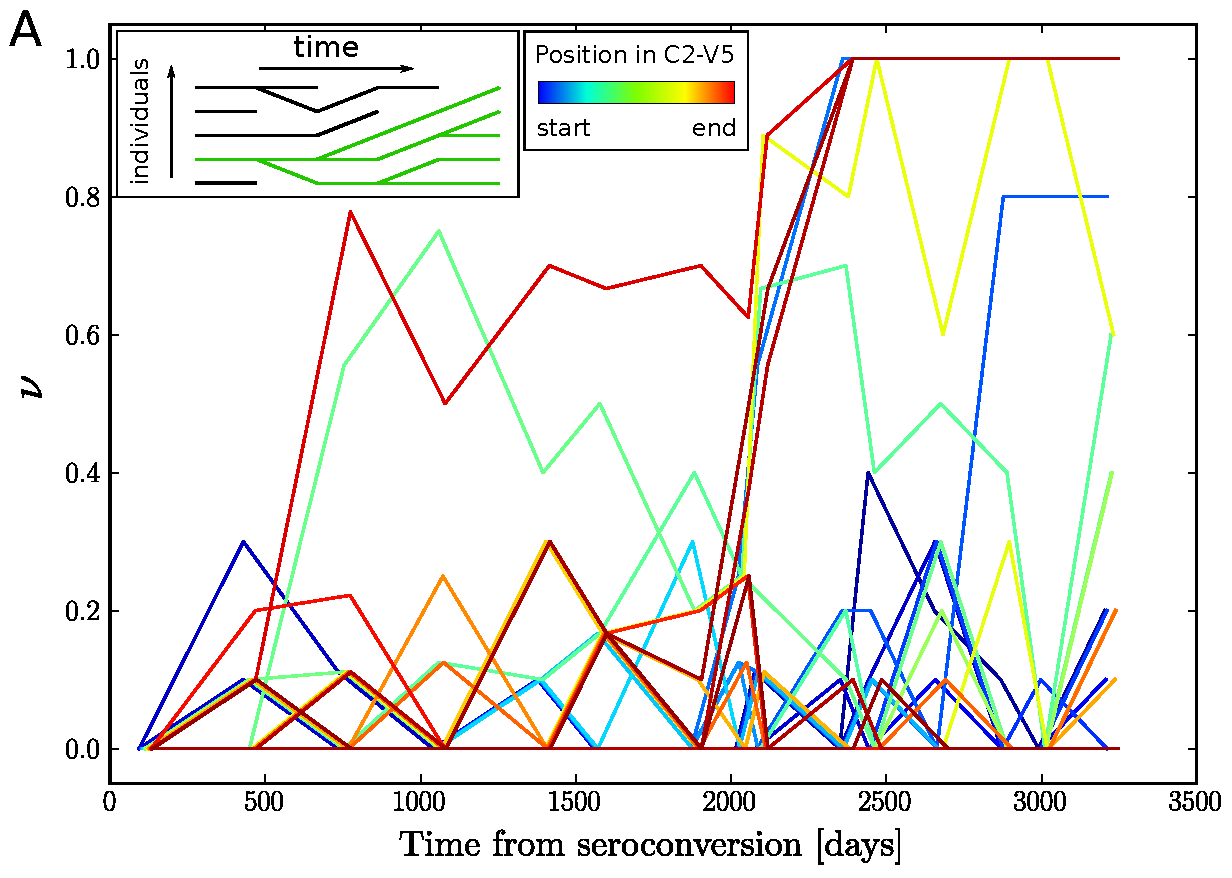
\includegraphics[width=\linewidth]{Shankarappa_allele_freqs_trajectories_syn_p1.pdf}
\label{fig:aftsyn}}\\
 \subfloat{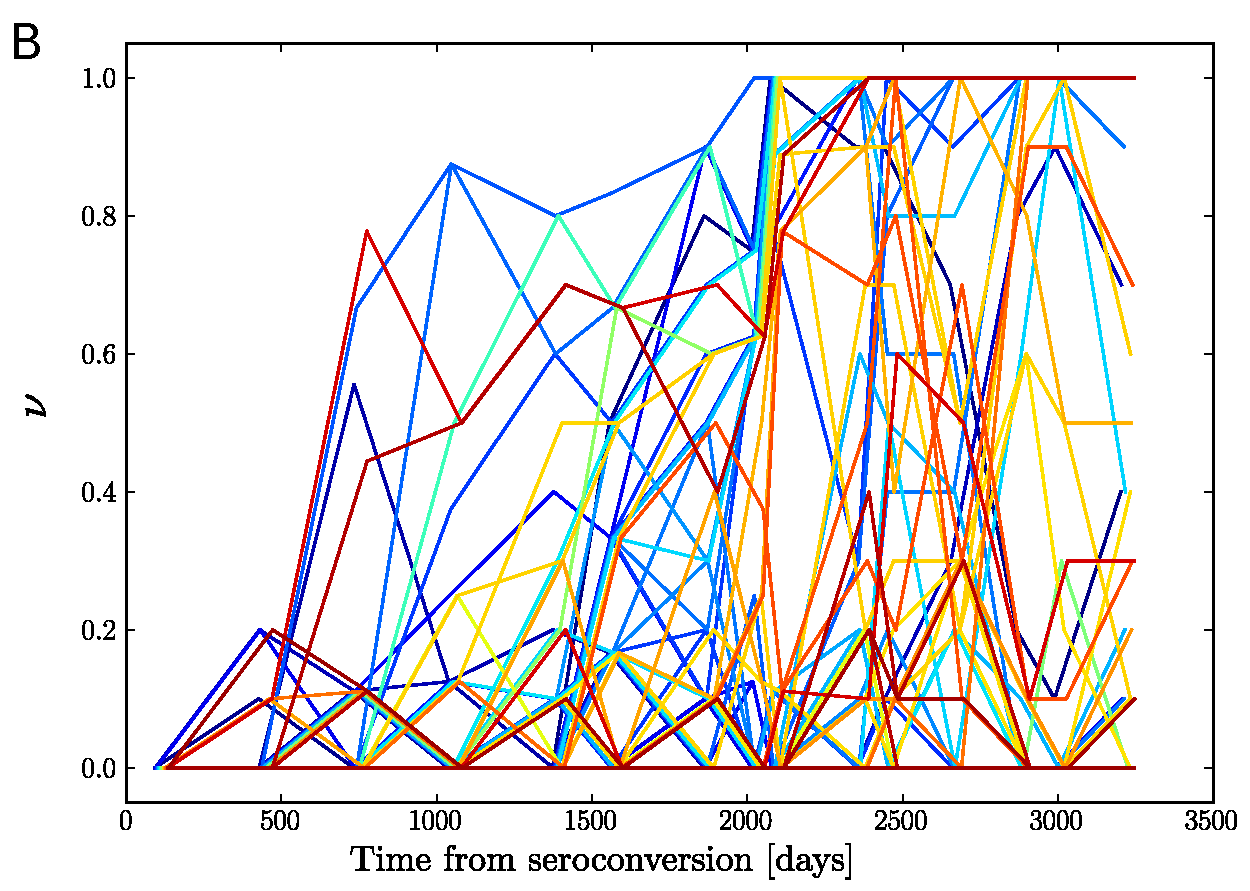
\includegraphics[width=\linewidth]{Shankarappa_allele_freqs_trajectories_nonsyn_p1.pdf}
\label{fig:aftnonsyn}}
\caption{Time series of frequencies of synonymous (A) and non-synonymous (B)
derived alleles in \env, C2-V5, from patient
1~\cite{shankarappa_consistent_1999}.
While many nonsynonymous mutations  fix, few synonymous
mutations do even though they are frequently observed at intermediate
frequencies. Colors indicate the position of the site along the C2-V5 region
(blue to red). Inset: the fixation probability $P_\text{fix}(\nu)$ of a neutral mutation
is simply the likelihood that the future common ancestor is currently carrying
it, i.e., its frequency $\nu$.}
\label{fig:aft}
\end{center}
\end{figure}

When interpreting these results for the fixation probabilities, it is important
to distinguish between random mutations and polymorphisms observed at a certain
frequency since the latter have already been filtered by selection.
A polymorphism could be beneficial to the virus and on its way to fixation. In
this case, we expect that it fixes almost surely given we see it at high
frequency. If, on the other hand, the polymorphism is deleterious it must have
gotten to high frequency by chance (genetic drift or hitchhiking), and
we expect that selection will drive it out of the population again. Hence our
observations suggest that many of the synonymous polymorphisms at intermediate
frequencies in the part of \env~that includes the hypervariable regions are
deleterious, while outside this regions polymorphisms are mostly roughly
neutral. Note that this does not imply that all synonymous mutations in this
region are neutral -- only those mutations observed at high frequencies, which
have been experiencing selection for some time already, tend to be neutral.

\begin{figure}
\begin{center}
\subfloat{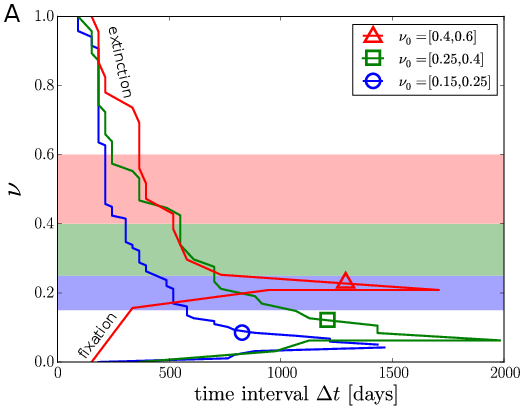
\includegraphics[width=0.9\linewidth]{fixation_times}
\label{fig:fixp1}}\\
\subfloat{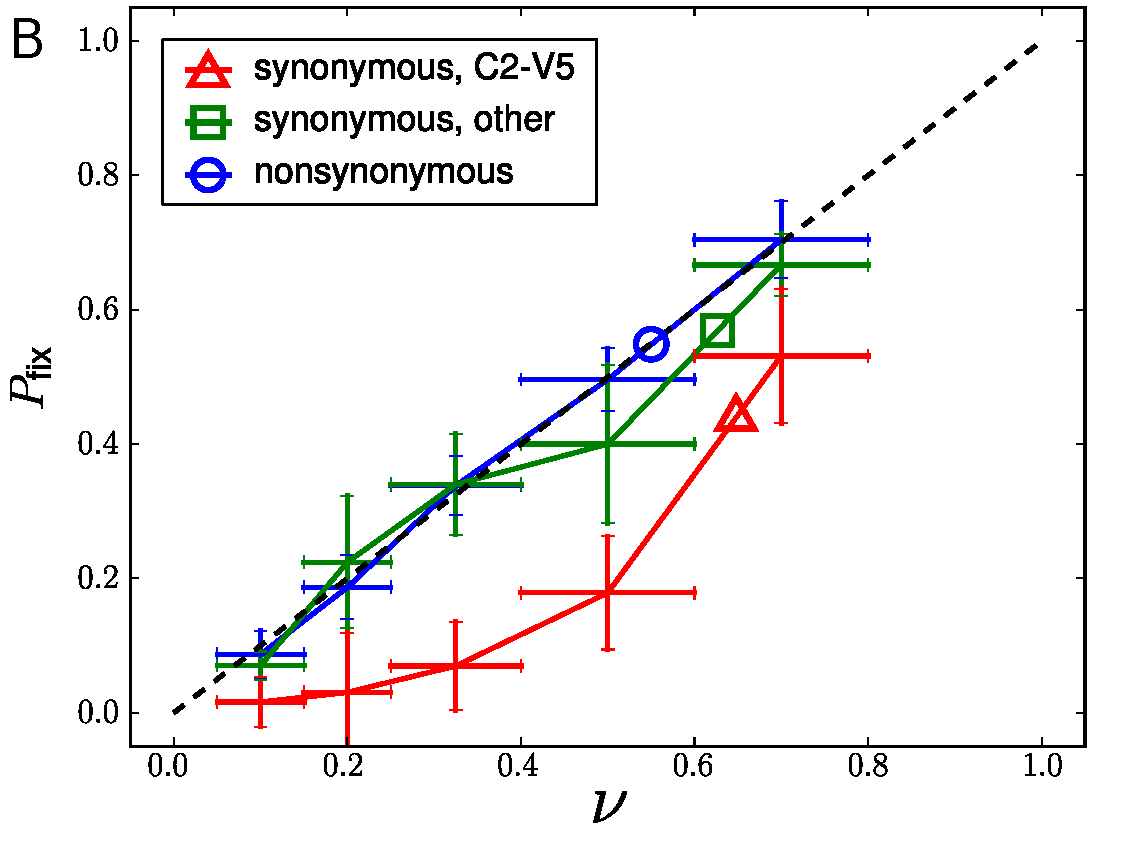
\includegraphics[width=0.9\linewidth]{fixation_probabilities}
\label{fig:fixp2}}
\caption{Fixation and loss of synonymous mutations.
Panel A) Time
course of loss and fixation of synonymous mutations observed in a frequency interval $\nu_0$. 
In each frequency interval, the  fraction of synonymous
mutations that ultimately fix is the fixation probability conditional on the
initial frequency.
Panel B) Fixation probability of derived synonymous
alleles as a function of $\nu_0$ in C2-V5 is below the neutral
expectation indicated by the diagonal line. This suppression is not
oberserved in other parts of {\it env} or for nonsynonymous mutations.
The horizontal error bars on the abscissa are bin sizes, the vertical ones the
standard deviation after 100 patient bootstraps of the data. Data from
Refs.~\cite{shankarappa_consistent_1999, bunnik_autologous_2008}.}
\label{fig:fixp}
\end{center}
\end{figure}

%%%%%%%%%%%%%%%%%%%%%%%%%%%%%%%%%%%%%%%%%%%%%%%%%%%%%%%%%%%%%%%%%%%%%%%%%
\subsection{Synonymous mutations in C2-V5 tend to disrupt conserved RNA stems}
%%%%%%%%%%%%%%%%%%%%%%%%%%%%%%%%%%%%%%%%%%%%%%%%%%%%%%%%%%%%%%%%%%%%%%%%%
One possible {\it a priori} explanation for lack of fixation of synonymous
mutations in C2-V5 are secondary structures in the viral RNA, the disruption of
which is deleterious to the virus.
It has been suggested early on that parts of the viral genome that have the
potential to form RNA stems are better conserved than the
remainder~\citep{forsdyke_reciprocal_1995,snoeck_mapping_2011}.

Recently, the propensity of nucleotides of the HIV genome to form base pairs has
been measured using the SHAPE assay (a biochemical reaction preferentially
altering unpaired bases)~\citep{watts_architecture_2009}. The SHAPE assay has
shown that the variable regions V1 to V5 tend to be unpaired, while the
conserved regions between those variable regions form stems. We partition all
synonymous alleles observed at intermediate frequencies above 10-15\% depending
on their final destiny (fixation or extinction). Subsequently, we align our
sequences to the reference NL4-3 strain used in
ref.~\citep{watts_architecture_2009} and assign them SHAPE reactivities. As
shown in \FIG{SHAPEA}, the reactivities of fixed
alleles (red histogram) are systematically larger than of alleles are lost (blue
) (Kolmogorov-Smirnov test, $P\approx 0.002$).
In other words, alleles that are likely to break RNA helices are also more
likely to revert and finally be lost from the population. The
average over all mutations that are not observed (green) lies between the
those that fix and those that get lost.
Note that, because of small differences in base pairing between the reference
strain NL4-3 and each patient's initial consensus sequence, this analysis is not
expected to be very sensitive, but very conservative.

To test the hypothesis that mutations in C2-V5 are lost because they break stems in the
conserved streches between the variable loops, we consider mutations in
variable loops and conserved parts separately. The biggest depression in
fixation probability is observed in the conserved stems, while the variable
loops show little deviation from the neutral signature, see \FIG{SHAPEB}. This
is consistent with important stem structures in conservered regions between loops.

In addition to RNA secondary structure, we have considered other possible
explanations for a fitness defect of synonymous mutations, in particular codon
usage bias (CUB). HIV is known to prefer A-rich codons over highly expressed
human codons~\citep{jenkins_extent_2003,kuyl_biased_2012}. We do not find,
however, any evidence for a contribution of average CUB to the ultimate fate of
synonymous alleles consistent with that HIV does not seem to adapt its codon
usage to its human host cells at the macroevolutionary level
\citep{kuyl_biased_2012}.


\begin{figure}
\begin{center}
\subfloat{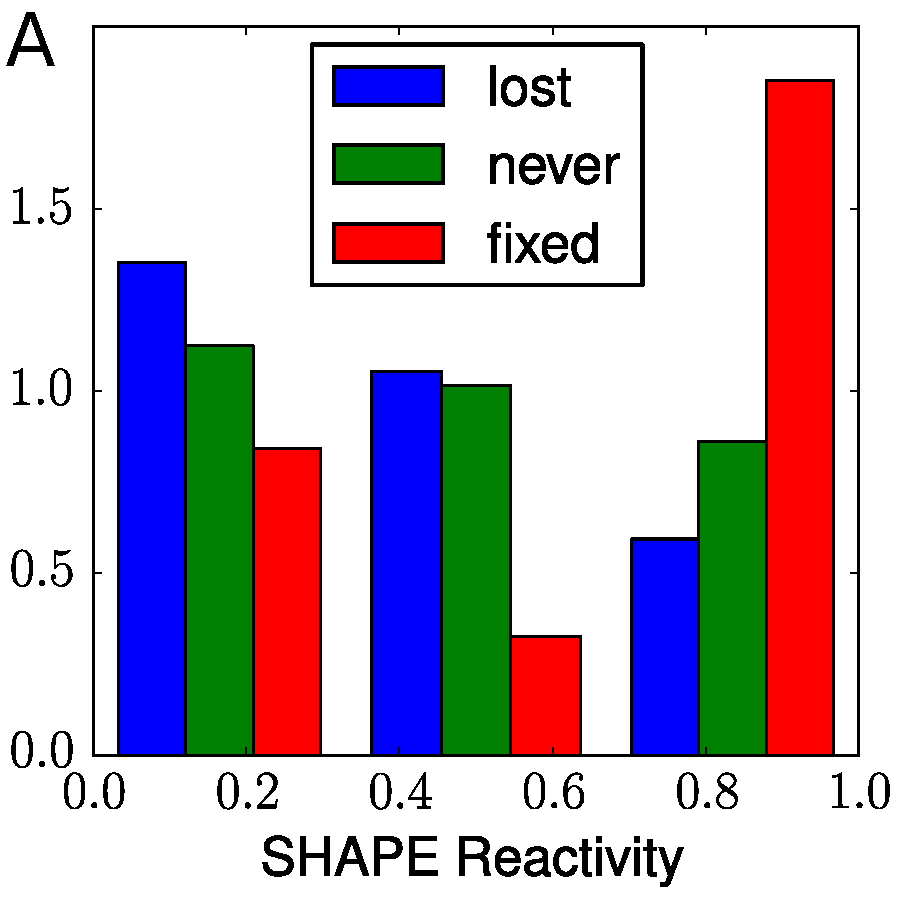
\includegraphics[height=0.46\linewidth]{reactivities_histograms_syn}
\label{fig:SHAPEA}}
\subfloat{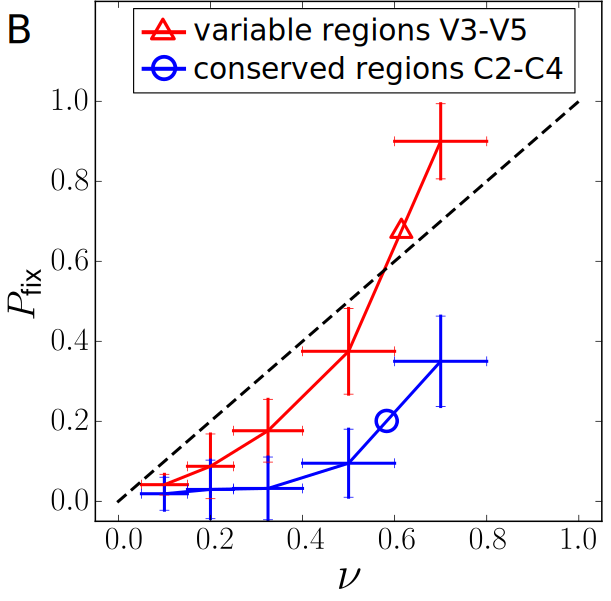
\includegraphics[height=0.46\linewidth]{fixation_probabilities_VnonV}\label{fig:SHAPEB}}
\caption{Permissible synonymous mutations have
high SHAPE reactivities.
Panel A) Synonymous substitions have
substantially higher SHAPE reactivities than mutations that reach frequencies above 15\%, but are
susequently lost (restricted to the regions V1-V5$\pm 100bp$ from each). This difference
is quantified by a cumulative histogram ($p=0.002$, Kolmogorov-Smirnov two 
sample test). Mutations that are never
observered show an intermediate distribution of SHAPE values.
Panel B) Fixation probability of synonymous mutations in C2-V5
separately for variable loops and the connecting conserved regions, that
harbor conserved RNA stems. As expected, fixation probability is lower inside
the conserved regions. Data from Refs.~\cite{shankarappa_consistent_1999,
bunnik_autologous_2008, liu_selection_2006}.}
\label{fig:SHAPE}
\end{center}
\end{figure}


%%%%%%%%%%%%%%%%%%%%%%%%%%%%%%%%%%%%%%%%%%%%%%%%%%%%%%%%%%%%%%%%%%%%%%%%%
\subsection{Deleterious mutations are brought to high frequency by hitchhiking}
%%%%%%%%%%%%%%%%%%%%%%%%%%%%%%%%%%%%%%%%%%%%%%%%%%%%%%%%%%%%%%%%%%%%%%%%%
While the observation that some fraction of synonymous mutations is deleterious
is not unexpected, it seems odd that we observe them at high population
frequency -- at least in some regions of the genome. The region of \env~in
which we observe deleterious mutations at high frequency undergoes frequent
adaptive changes to evade recognition by neutralizing 
antibodies~\cite{williamson_adaptation_2003,richman_rapid_2003}. Due to the 
limited amount of recombination in HIV~\cite{neher_recombination_2010,batorsky_estimate_2011},
deleterious mutations that are linked to adaptive variants can reach high
frequency. This process is known as hitchhiking \citep{smith_hitch-hiking_1974}
or genetic draft \citep{gillespie_genetic_2000,neher_genetic_2011}.
Hitchhiking is  apparent in \FIG{aft}, that shows that many mutations
change rapidly in frequency as a flock. 

The approximate magnitude of the deleterious effects can be estimated from
\FIG{fixp1}, that shows the distribution of times for synonymous
alleles to reach the fix or get lost starting from intermediate frequencies. The
typical time to loss is of the order of 500 days. If this loss is driven by the
deleterious effect of the mutation, this corresponds to deleterious effects of
roughly $s_d \sim - 0.002$ per day.

\begin{figure}
\begin{center}
\subfloat{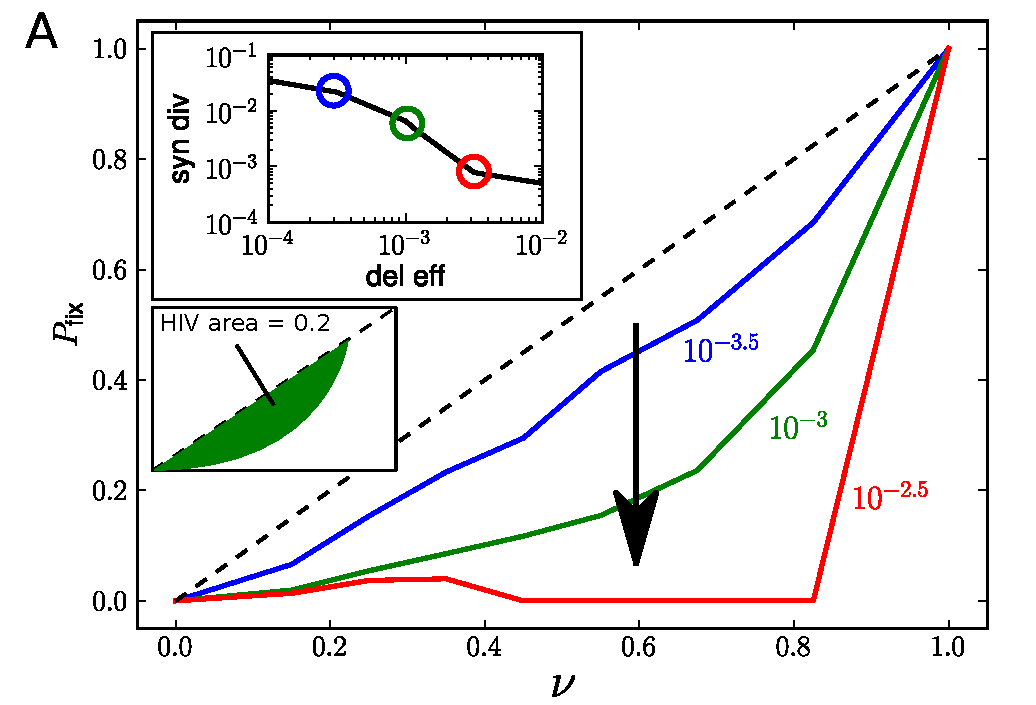
\includegraphics[width=\linewidth]{simulations_graduallydel.pdf}
\label{fig:simfixpvar}}\\
\subfloat{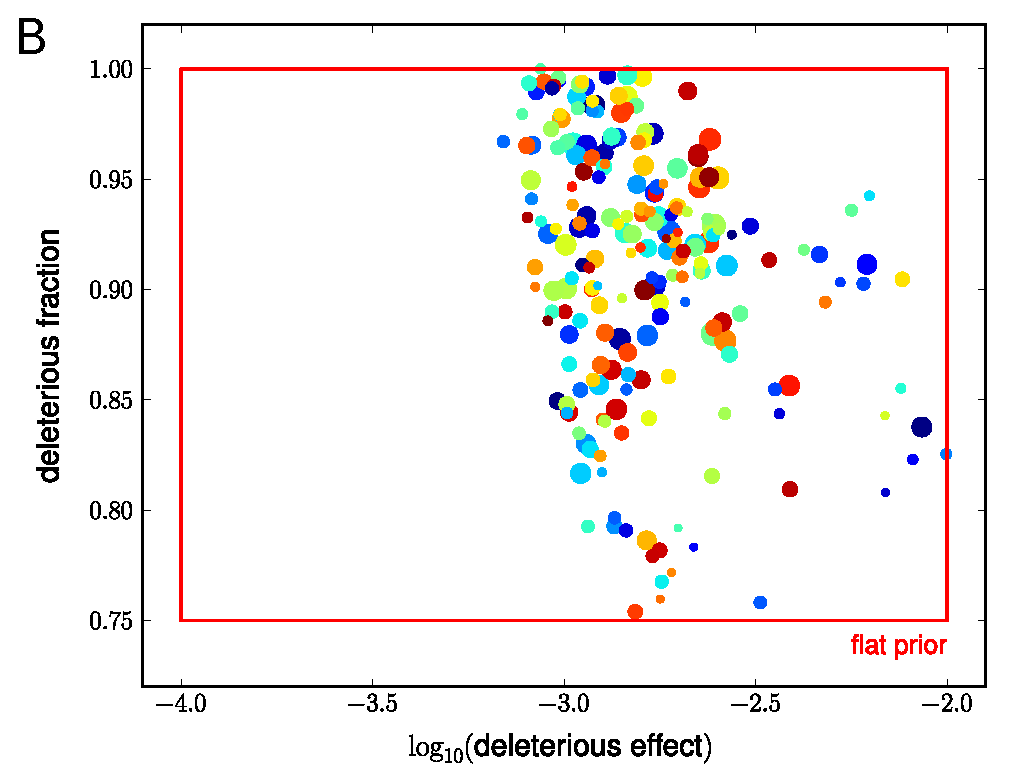
\includegraphics[width=\linewidth]{simulations_syn.pdf}
\label{fig:simsfig}}
\caption{Distribution of selection coefficients on synonymous sites. Panel A)
The depression in $P_\text{fix}$ depends on the deleterious effect size 
of the synonymous alleles. This parameter also reduces synonymous
diversity, measured by the probability of a derived allele to be found at
intermediate frequencies $P_\text{interm}$ (first inset).
Panel B) To assess the parameter space that affects synonymous fixation and
diversity, we run many simulations with random parameters for deleterious effect
size, fraction of deleterious synonymous sites, average size of escape
mutations (color, blue ($10^{-2.5}$) to red ($10^{-1.5}$)), and rate of
introduction of new epitopes (marker size, from $10^{-3}$ to $10^{-2}$ per
generation). Mostly simulations with small deleterious effects and relatively
high deleterious fractions of synonymous mutations reproduce synonymous the
fixation probability and diversity observed in patients. Parameters are chosen
from uninformed prior distributions in the indicated window (see methods).}
\label{fig:simheat}
\end{center}
\end{figure}

To get a better idea of the range of parameters that are compatible with the
observations and our interpretation, we performed computer simulations of
evolving viral populations assuming a mix of positive and purifying selection
and rare recombination.
For this purpose, we use the simulation package FFPopSim, which includes a
module dedicated to intrapatient HIV evolution~\citep{zanini_ffpopsim:_2012}. 
For each simulation run, we specify the deleterious effect of synonymous
mutations, the fraction of synonymous mutations that are deleterious, the
escape rate of adaptive non-synonymous mutations and the frequency of new
escapes. Note that the escape rate is sum of two factors: (i) the beneficial
effect due to the ability to evade the immune system minus (ii) the fitness
cost of the mutation in terms of structure, stability, etc. Net escape rates
in chronic infections have been estimated to be on the order of 
$s_a = 0.01$ per day~\citep{neher_recombination_2010, Asquith}.
\comment{Asquith??}

\FIG{simfixpvar} shows simulations results for the fixation probability and the
synonymous diversity for different deleterious effects of synonymous mutations. 
We quantify synonymous diversity,$P_\text{interm}$, as the fraction of sites
with an allele at frequency $0.25 < \nu < 0.75$. The synonymous diversity
observed in patient data is indicated in the figure.
To quantify the depression of the fixation probability, we calculate
the area between the measured fixation probability and the diagonal, which is
the neutral expectation (\FIG{simfixpvar}, lower inset). If no fixation happens,
the area will be $-0.5$; if every mutation fixes, we will measure 
$A= 0.5$. In HIV, we find $A_\text{syn} \sim -0.2$  for
synonymous changes and $A_\text{nonsyn} \sim 0$ for nonsynonymous changes.

In the three simulations shown in \FIG{simfixpvar}, the fixation probability of
synonymous alleles decreases from the neutral expectation ($A_\text{syn} \sim 0$) to zero
($A_\text{syn} \sim -0.5$) as their fitness effect
worsens; the synonymous diversity plummets as well, as it is harder for
deleterious mutations to reach the frequency threshold of 0.25.

To map the parameter range of the model that is compatible with the data, we
repeatedly simulated the evolution with random choices for the parameters in
certain bounds, see \FIG{simsfig}.
Among all simulations, we select the ones that show $A_\text{syn}$ and
$P_\text{interm}$ as observed in the data, i.e., a large depression in fixation
probability of synonymous mutations but, simulteneously, a moderately high
synonymous diversity. Specifically, \FIG{simsfig} shows parameter combinations
for which we found $A_\text{syn} < -0.15$ and $0.0025 < P_\text{interm} <
0.010$. These conditions indicate that a high fraction ($\gtrsim 0.8$) of
deleterious sites has to be deleterious with effect size $|s_d| \sim 0.002$. 
This result fits well the expectation based on the fixation/extinction times above (see \FIG{fixp1}).
The results are plausible:
(i) a substantial depression in $\pfix$ requires pervasive deleterious
mutations, otherwise the majority of observed polymorphisms are neutral and no
depression is observed; (ii) in order to hitchhike, the deleterious effect size
has to be much smaller than the escape rate, otherwise the double mutant has
little or no fitness advantage; (iii) mutations with a deleterious effect
smaller than approximately $0.001$ behave neutrally consistent with the typical
coalescent times observed in HIV.

As long as only features of synonymous mutations are filtered, as performed
above, the two nonsynonymous parameters, escape rate
and rate of appearance of epitopes, are little constrained as is apparent in
\FIG{simsfig} from the variety of sizes and colors indicating these parameters.
In most of these simulations, however, nonsynonymous mutations almost always fix once they reach high frequencies
-- their nonsynonymous fixation area is well above zero. This is incompatible
with the blue line in \FIG{fixp}: in an HIV infection, nonsynonymous
mutations at high frequency often disappear again, even though many are at
least transiently beneficial. Inspecting the trajectories of nonsynonymous
mutations suggests the rapid rise and fall of many alleles. We test two possible
mechanisms that are biologically plausible and could explain the transient rise
of nonsynonymous mutations: time-dependent selection and within-epitope
competition.

The former hypothesis can be formulated as follows: if the immune system
recognizes the escape mutant before its fixation, the mutant might cease to be
beneficial and disappear soon, despite its quick initial rise in frequency. In support of this idea,
\citet{richman_rapid_2003, bunnik_autologous_2008} report antibody responses to
escape mutants. These respones are delayed by a few months, roughly matching the
average time needed by an escape mutant to rise from low to high frequency.
In the alternative hypothesis, several different escape
mutations within the same epitope might arise almost simultaneously and start to
spread. Their benefits are not additive, because each of them is
essentially sufficient to escape. As a consequence, several escape mutations rise to
high frequency rapidly, while the one with the smallest cost in terms of replication,
packaging, etc.~is most likely to eventually fix. The emergence of
multiple sweeping nonsynonymous mutations in real HIV infections has been 
shown~\citep{moore_limited_2009, bar_early_2012}.
We tested both hypotheses in our simulation framework and they both result
in a reduced, neutral-like fixation probability while maintaining a high
rate of substitutions, compatible with observations in patient data (see
supplementary materials).
The two scenarios are not exclusive and possibly both important in HIV
evolution.

%%%%%%%%%%%%%%%%%%%%%%%%%%%%%%%%%%%%%%%%%%%%%%%%%%%%%%%%%%%%%%%%%%%%%%%%%
\section{Discussion}
%%%%%%%%%%%%%%%%%%%%%%%%%%%%%%%%%%%%%%%%%%%%%%%%%%%%%%%%%%%%%%%%%%%%%%%%%
Despite several known functional roles for RNA secondary structure in the HIV
genome, synonymous mutations are often used as approximately neutral markers in
evolutionary studies of viruses. By analyzing the fate of mutations in
longitudinal data of HIV \env{} evolution, we have shown that the majority of
synonymous mutations in the conserved regions C2-C5 of the \env~gene are deleterious.
Comparison with recent biochemical studies of binding propensity of bases in RNA
genome indicates that these mutations are deleterious, at least in part, because
they disrupt stems in RNA secondary structures. Computational modelling
shows that these mutations can be brought to high frequency through
linkage to adaptive mutations.

The fixation and extinction times and probabilities represent a rich and simple
summary statistics useful to characterize longitudinal sequence data and compare
to models via computer simulations. Although several recent publications have
pointed out that synonymous changes in HIV can be
deleterious~\citep{lemey_synonymous_2007, ngandu_extensive_2008}, our analysis
is much more direct, as we rely neither on phylogenetic tree reconstruction nor
on macroevolutionary models. A method that is similar to ours {\it in spiritu}
has been recently used in a longitudinal study of influenza
evolution~\citep{strelkowa_clonal_2012}. The propagators suggested in that
article, however, represent ratios between nonsynonymous and synonymous
mutations.  The latter is used as an approximately neutral control; this method
can therefore not be used to investigate synonymous changes themselves. A
functional significance of the insulating RNA structure stems between the
hyper-variable loops has also been proposed
previously~\citep{watts_architecture_2009, sanjuan_interplay_2011} and conserved
RNA structures exist in different parts of the HIV
genome~\citep{ngandu_extensive_2008}. Our analysis is nonetheless much more
direct and is able to quantify the fitness effect of RNA structure within single
infections. The main limitations of our approach are the following: (i) it
requires longitudinal data, most of which focuses on \env{} only; and (ii) we
only expect to see deleterious synonymous mutations at high frequencies if they
are linked to repeated adaptive substitions. Otherwise, most synonymous
polymorphisms remain at low frequencies and can only be observed by deep
sequencing methods. We indeed plan to exploit next-generation sequencing
technologies to assess synonymous diversity at the level of rare variants in
future studies.

Contrary to na\"ive expectations, the adaptive escape mutations do not seem to be
unconditionally beneficial. Otherwise we would observe almost sure fixation of
nonsynonymous mutations once they reach intermediate frequencies. Instead, we
find that the fixation probability of nonsynonymous mutations is roughly given
by its frequency. There are several possible explanations for this observation. 
Similar to synonymous mutations, the majority of nonsynonymous mutations could
be weakly deleterious and the adaptive and deleterious parts conspire to yield
the neutral-like averaged fixation probability. We consider this possibility
inplausible since the amino-acid sequence outside the variable loops is much
more conserved that the synonymous positions, suggesting that the majority of
the nonsynonymous mutations is much more deleterious (see supplementary
materials). 

Alternatively, the lack of fixation could be due to time dependent environment
through an immune system that is catching up, or competition between mutations
that mediate escape within the same epitope. We explore both of these
possibilities and find that both produce the desired effect. Furthermore, there
is experimental evidence in support of both of these hypotheses. Serum from HIV
infected individuals tyically neutralizes the virus that dominated the
population a few (3-6) month ago \citep{richman_rapid_2003}. This suggests that
escape mutations cease to be beneficial after a few months and might revert if
they come with a fitness cost. Deep sequencing of regions of \env{} after
antibody escape have revealed multiple escape mutations in the same epitope
\citep{moore_limited_2009, bar_early_2012}. Presumably, each one of these
mutations is sufficient for escape but most combinations of them don't provide
any additional benefit to the virus. Hence only one mutation will spread and the
others will be driven out of the population although they transiently reach high
frequencies. The rapid emergence of multiple escape mutations in the same
epitope implies a large population size that explores all necessary point
mutations rapidly. A similar point has been made recently by Boltz {\it et al.}
in the context of preexisting drug resistance
mutations~\citep{boltz_ultrasensitive_2012}. 

The observed hitchhiking highlights the importance of linkage due to infrequent
recombination for the evolution of HIV
\citep{neher_recombination_2010,batorsky_estimate_2011,
josefsson_majority_2011}. The recombination rate has been estimated to be on the
order of $\rho = 10^{-5}$ per base and day. It takes roughly $t_{sw} =
\epsilon^{-1} \log \nu_0$ generations for escape mutation with escape rate
$\epsilon$ to rise from an initially low frequency $\nu_0\sim \mu$ to frequency
one. This implies that a region of length $l = (\rho t_{sw})^{-1} = \epsilon /
\rho \log \nu_0$ remains linked to the adaptive mutation. With $\epsilon=0.01$,
we have $l\approx 100$ bases. Hence we expect strong linkage between the
variable loops and the intervening sequence, but none far beyond the variable
regions, consistent with the lack of signal outside of C1-V5. In case of much
stronger selection -- such as observed during early CTL escape or drug
resistance evolution -- the linked  region is of course much larger
\citep{nijhuis_stochastic_1998}.

Our results emphasize the inadequacy of independent site models of HIV evolution
and the common assumption that selection is time independent or additive. If
genetic variation is only transiently beneficial, existing estimates of the
strength of selection \citep{neher_rate_2010,batorsky_estimate_2011} could be
substantial underestimates.

%%%%%%%%%%%%%%%%%%%%%%%%%%%%%%%%%%%%%%%%%%%%%%%%%%%%%%%%%%%%%%%%%%%%%%%%%
\section{Methods}
%%%%%%%%%%%%%%%%%%%%%%%%%%%%%%%%%%%%%%%%%%%%%%%%%%%%%%%%%%%%%%%%%%%%%%%%%
\subsection{Sequence data collection}
%%%%%%%%%%%%%%%%%%%%%%%%%%%%%%%%%%%%%%%%%%%%%%%%%%%%%%%%%%%%%%%%%%%%%%%%%
Longitudinal intrapatient viral RNA sequences were collected from published
studies~\citep{shankarappa_consistent_1999, liu_selection_2006,
bunnik_autologous_2008} and downloaded from the Los Alamos National Laboratory
(LANL) HIV sequence database~\citep{LANL2012}. The samples from some patients
show substantial population structure and were discarded (see supplementary
materials); a total of 11 patients with 4-23 time points each and approximately 10
sequences per time point were analyzed. The time intervals between two
consecutive sequences ranged from 1 to 34 months, most of them between 6 and 10
months.

%%%%%%%%%%%%%%%%%%%%%%%%%%%%%%%%%%%%%%%%%%%%%%%%%%%%%%%%%%%%%%%%%%%%%%%%%
\subsection{Sequence analysis}
%%%%%%%%%%%%%%%%%%%%%%%%%%%%%%%%%%%%%%%%%%%%%%%%%%%%%%%%%%%%%%%%%%%%%%%%%
The sequences were translated and the resulting amino-acid sequences aligned
using Muscle~\citep{edgar_muscle:_2004} to each other and the NL4-3 reference
sequences separately for each patient. Within each patient, the consensus
nucleotide sequence at the first time point was used to classify alleles as
``ancestral'' or ``derived'' at all sites. Sites that include large
frequencies of gaps were excluded from the analysis to avoid artefactual
substitutions due to alignment errors. Allele frequencies at different time
points were extracted from the multiple sequence alignment.

A mutation was considered synonymous if it did not change the amino acid
corresponding to the codon, and if the rest of the codon was in the ancestral
state. Codons with more than one mutation were discarded. Slightly different
criteria for synonymous/nonsynonymous discrimination yielded similar results.

%%%%%%%%%%%%%%%%%%%%%%%%%%%%%%%%%%%%%%%%%%%%%%%%%%%%%%%%%%%%%%%%%%%%%%%%%
\subsection{Fixation probability and secondary structure}
%%%%%%%%%%%%%%%%%%%%%%%%%%%%%%%%%%%%%%%%%%%%%%%%%%%%%%%%%%%%%%%%%%%%%%%%%
For the estimate of times to fixation/extinction, polymorphisms were
binned by frequency and the time to reaching the first boundary (fixation or
extinction) was stored. The fixation probability was determined as the long-time
limit of the resulting curves. Mutations that reached high frequency but neither
fixed nor got extinct were classified as ``floating'' and not analyzed further.

The SHAPE scores quantifying the degree of base pairing of individuals sites in
the HIV genome were downloaded from the journal
website~\citep{watts_architecture_2009}.
Where possible, SHAPE reactivities were assigned to sites in the multiple
sequence alignments for each patient through the alignment to the sequence
of the NL4.3 virus used in ref.~\citep{watts_architecture_2009}. Problematic
assignments in indel-rich regions were excluded from the analysis.

The variable loops and flanking regions were identified manually starting from
the annotated reference HXB2 sequence from the LANL HIV database~\citep{LANL2012}. A
similar approach was used to label the C2-V5 region sequenced in
ref.~\citep{shankarappa_consistent_1999}.

%%%%%%%%%%%%%%%%%%%%%%%%%%%%%%%%%%%%%%%%%%%%%%%%%%%%%%%%%%%%%%%%%%%%%%%%%
\subsection{Computer simulations}
%%%%%%%%%%%%%%%%%%%%%%%%%%%%%%%%%%%%%%%%%%%%%%%%%%%%%%%%%%%%%%%%%%%%%%%%%
Computer simulations were performed using
FFPopSim~\citep{zanini_ffpopsim:_2012}. Both full-length HIV genomes and
\env{}-only simulations were performed and yielded comparable results. In each
simulation, four random parameters were drawn form prior distributions: (i)
fraction of deleterious synonymous sites (flat between 0.75 and 1.0); (ii)
deleterious effect at those sites (exponential between $10^{-4}$ and $10^{-2}$);
(iii) average beneficial effect of an escape mutation (exponential between
$10^{-2.5}$ and $10^{-1.5}$); (iv) rate of introduction of new epitopes
(exponential between $10^{-3}$ and $10^{-2}$ per generation). After these four
parameters were fixed, the simulation started. All the deleterious synonymous
sites had the same fitness effect (variations were tested and produced the same
results), no epitopes (i.e. no escape mutations) were initially present, and the
population was isomorphic.
After 30 generations of burn-in to create genetic diversity, new epitopes
were introduced at a constant rate (as specified above). Each time such an
epitope was actually introduced, its fitness advantage was drawn from an
exponential distribution with fixed average value (as specified above).
For the models with competition within epitopes, a complex epistatic fitness
landscape was manually crafted, in which each single mutant provides the whole
beneficial effect of escape. For the models with time-dependent selection due to
the immune system catching up, the beneficial effect of an escape mutation was
reverted at random times after it had appeared, according to its integrated allele
frequency (see supplementary materials for more details).

For each set of parameters, fixation probabilities and probabilities of
synonymous polymorphisms $P_\text{interm}$ were calculated as averages over
approximately 100 repetitions (with different random seeds).

The areas below or above the neutral fixation probability (diagonal line)
were estimated from the binned fixation probabilities using linear
interpolation between the bin centers. This measure is sufficiently precise for
our purposes.

%%%%%%%%%%%%%%%%%%%%%%%%%%%%%%%%%%%%%%%%%%%%%%%%%%%%%%%%%%%%%%%%%%%%%%%%%
\subsection{Methods availability}
%%%%%%%%%%%%%%%%%%%%%%%%%%%%%%%%%%%%%%%%%%%%%%%%%%%%%%%%%%%%%%%%%%%%%%%%%
All analysis and computer simulation scripts, as well as the sequence alignments
used, are available for download.

%%%%%%%%%%%%%%%%%%%%%%%%%%%%%%%%%%%%%%%%%%%%%%%%%%%%%%%%%%%%%%%%%%%%%%%%%
\section*{Acknowledgements}
%%%%%%%%%%%%%%%%%%%%%%%%%%%%%%%%%%%%%%%%%%%%%%%%%%%%%%%%%%%%%%%%%%%%%%%%%
We are grateful for stimulating discussions with Jan Albert and Trevor Bedford.
This work is supported by the ERC starting grant HIVEVO 260686.

%%%%%%%%%%%%%%%%%%%%%%%%%%%%%%%%%%%%%%%%%%%%%%%%%%%%%%%%%%%%%%%%%%%%%%%%%
\bibliographystyle{natbib}
\bibliography{bib}
%%%%%%%%%%%%%%%%%%%%%%%%%%%%%%%%%%%%%%%%%%%%%%%%%%%%%%%%%%%%%%%%%%%%%%%%%
\end{document}
%%%%%%%%%%%%%%%%%%%%%%%%%%%%%%%%%%%%%%%%%%%%%%%%%%%%%%%%%%%%%%%%%%%%%%%%%

